\documentclass[a4paper,8pt,twocolumn]{article}
\usepackage[UTF8]{ctex}
\usepackage{graphicx}
\usepackage{fancyhdr}
\usepackage{amsmath}
\usepackage[
  left=2cm, 
  right=2cm,
  top=1.5cm,
  bottom=2.5cm
]{geometry}
\usepackage{pgfplots}
\usepackage{pgfplotstable}
\pgfplotsset{compat=1.18}
\usepackage{siunitx} % 用于正确显示单位

\begin{document}

\title{
  \textbf{\huge G1 温度测控仪的设计与组装}}
\author{
  黄雨~24352027\\
\small 中山大学物理学院~广东~广州
}

\maketitle

\section{实验目的}
 \noindent
 1、学习数显温度计和温度控制仪的工作原理。\\
 2、利用 PT100（或Cu50）金属热敏电阻、LM35 型、AD590 型等三种典型温度传感器组装温度测试和控制电路。\\

\section{实验用具}
 \noindent
 致冷/加热温度控制仪、直流稳压稳流电源、数字万用表、温度传感器、九孔板、导线等。\\

\section{实验原理}
 本实验利用LM35电压型温度传感器作为感温元件，组装温度测试和控制电路。
 \subsection{温度传感器}
  LM35 电压型集成电路温度传感器。输出电压大小与温度成正比，线性度极好，准确度一般为$\pm 0.5\,^{\circ}\text{C}$。内部有激光校准电路，保证了极高的准确度及一致性。被测温度与输出电压的关系可写为
  \[ T(^{\circ}\text{C}) = V_o / K_v \qquad \]
  其中，$K_v$ 称为电压温度系数，$K_v = 10.0\,\text{mV} \cdot {^{\circ}\text{C}}^{-1}$。
 \subsection{温度测控仪电路}
  \noindent
  \textbf{基于LM35型温度传感器的数显温度测控仪}\\
  图\ref{3.1}所示电路中测试点\textcircled{1}的电压随温度线性变化，由上式确定。调节 $R_X$，使测试点\textcircled{2}的电压为 $0.800\text{ V}$ (即控温 $80^\circ\text{C}$)。温度低于设置的温度时，测试点\textcircled{4}和\textcircled{5}为高电平，继电器开关 $K$ 吸合，开始加热；温度高于设置温度时，测试点\textcircled{4}和\textcircled{5}为低电平，继电器开关 $K$ 断开，停止加热。\\
  \begin{figure}[ht] 
    \centering
    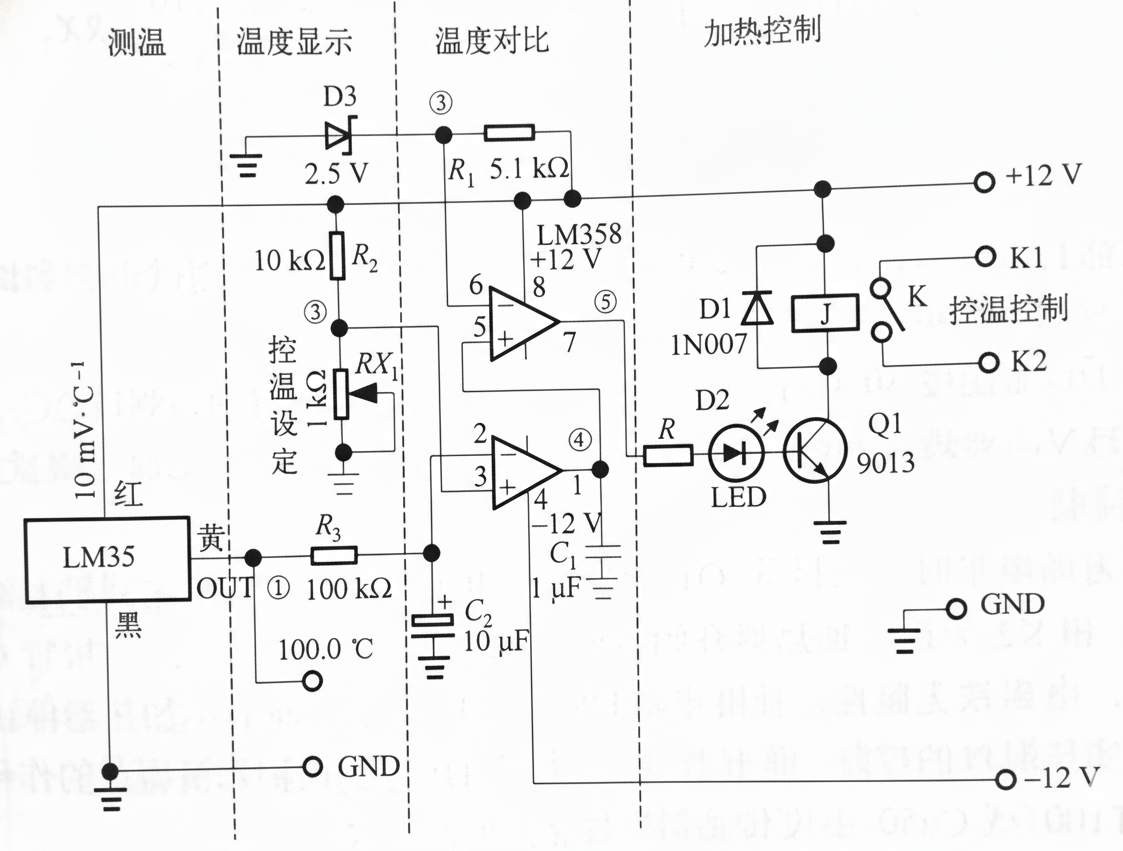
\includegraphics[width=0.5\textwidth]
    {3.1.png} 
    \caption{基于 LM35 型温度传感器的数显温度测控仪电路}
    \label{5.1} 
  \end{figure}\\

\section{实验装置}
 为验证上述电路是否正确工作，采用实验 A4 所用致冷/加热温度控制仪和恒温金属浴进行温度传感和控制。采用双路直流稳压电源提供$\pm12\text{V}$的电压，采用$5-3/4$位精度的数字万用表测量电压并等效为温度值。采用九孔板和插拔式电子元器件组装电路。

\section{实验内容及步骤}
 \noindent
 基于 LM35 电流型温度传感器的数显温度测控仪
  \begin{enumerate}
   \item 参照图\ref{3.1}组装电路，在室温时测量并记录 5 个测试点的对地电压。
   \item 改变温度，测量数字电压表测量值随温度变化关系曲线。
   \item 根据曲线确定 $80^\circ\text{C}$ 对应的电压，将温度控制电压设置为该值。
   \item 观察电路工作状态，记录继电器通、断时对应的温度，以及受控温金属浴温度波动的最小值 $T_{\min}$ 和最大值 $T_{\max}$，则控温精度为$$\Delta T = T_{\max} - T_{\min}$$
   \item 详述电路的工作过程。
  \end{enumerate}

\section{实验数据}
 \subsection{实物图}
  完成组装的实验装置如下图所示
  \begin{figure}[ht] 
    \centering
    
\includegraphics[width=0.4\textwidth]
    {4.1.png} 
    \caption{实物图}
    \label{4.1} 
  \end{figure}\\

 \subsection{5个测试点的对地电压}
  \begin{table}[h]
  \centering
   \begin{tabular}{|c|c|}
    \hline
    $\text{测试点}$ & $U/mV$ \\ 
    \hline
    $1$ & $302.260$ \\ 
    \hline
    $2$ & $478.260$ \\
    \hline
    $3$ & $2501.53$ \\
    \hline
    $4$ & $10367.6$ \\
    \hline
    $5$ & $10365.8$ \\
    \hline
  \end{tabular}
  \caption{测试点的对地电压}
  \label{Date_1}
 \end{table}

 \subsection{数字电压表测量值随温度变化关系曲线}
   \begin{tikzpicture}
    \begin{axis}[
        title={数字电压表测量值随温度变化关系},
        xlabel={$T/^\circ\text{C}$},
        ylabel={U/mV},
        xmin=10, xmax=100,
        ymin=100, ymax=900,
        grid=major, % 显示网格
        legend style={at={(0.5,-0.2)},anchor=north} % 图例位置
    ]

    % 1. 绘制原始数据点 (散点图)
    \addplot[
        only marks,      % 只显示标记，不连线
        mark=*,          % 使用实心圆作为标记
        blue             % 颜色为蓝色
    ] table {
        % 您的数据 (X Y)
        10.1 121.96
        15.0 164.16
        20.0 195.76
        25.0 249.78
        30.0 286.60
        35.0 339.22
        40.0 384.55
        45.0 436.37
        50.0 477.47
        55.0 570.80
        60.0 572.73
        65.0 620.00
        70.0 667.48
        75.0 714.48
        80.0 761.05
        85.0 807.11
        90.0 851.38
        95.0 900.20
        96.0 860.26
        100.0 871.96
    };
    \addlegendentry{原始数据};

    % 2. 绘制线性拟合线
    % \addplot+[<选项>] table[<键值对>] {数据} 
    % 键值对中的 'y={create col/linear regression}' 告诉 pgfplots 进行线性拟合
    \addplot[
        red,             % 拟合线颜色为红色
        very thick       % 拟合线较粗
    ] table[
        y={create col/linear regression}, % 核心命令：进行线性拟合
        % meta=y          % 这行是可选的，确保拟合使用的是 Y 轴数据
    ] {
        % 再次提供您的数据
        10.1 121.96
        15.0 164.16
        20.0 195.76
        25.0 249.78
        30.0 286.60
        35.0 339.22
        40.0 384.55
        45.0 436.37
        50.0 477.47
        55.0 570.80
        60.0 572.73
        65.0 620.00
        70.0 667.48
        75.0 714.48
        80.0 761.05
        85.0 807.11
        90.0 851.38
        95.0 900.20
        96.0 860.26
        100.0 871.96
    };
    \addlegendentry{线性拟合};

    % 可选：显示拟合方程 (需要手动计算或在外部计算)
    % 假设拟合方程为 y = 1.9x + 0.1
    % \node at (axis cs: 4, 1.5) [anchor=west] {$y = 1.9x + 0.1$};
    % 格式化斜率和截距，保留两位小数
    

    \end{axis}
\end{tikzpicture}\\
由图，$80^\circ\text{C}$对应的电压为$761.05~mV$

\subsection{温度控制}
 将温度控制电压设置为$761.05~mV$后，反复三次实验，得到数据如\ref{Date_2}所示：\\
 \begin{table}[h]
  \centering
   \begin{tabular}{|c|c|c|c|}
    \hline
    $T_\text{通}/^\circ\text{C}$ & $76.1$ & $80.0$ & $79.0$ \\ 
    \hline
    $T_\text{断}/^\circ\text{C}$ & $80.4$ & $79.7$ & $80.2$ \\
    \hline
    $T_\text{max}/^\circ\text{C}$ & $82.9$ & $81.6$ & $82.7$ \\
    \hline
    $T_\text{min}/^\circ\text{C}$ & $75.1$ & $78.1$ & $76.9$ \\
    \hline
  \end{tabular}
  \caption{控温数据}
  \label{Date_2}
 \end{table}\\
 计算不确定度时，由于数字万用表非常精确，B类不确定度可忽略，不确定度分析如下：\\
 \begin{eqnarray*}
    \overline{T_\text{通}} = \frac{1}{3}\sum_{i = 0}^{3}T_\text{通,i} = 78.367^\circ\text{C} \\
    \overline{T_\text{断}} = \frac{1}{3}\sum_{i = 0}^{3}T_\text{断,i} = 80.1^\circ\text{C} \\
 \end{eqnarray*}
 \begin{equation*}
    S_{T_\text{通}} = \sqrt{\frac{1}{3\times2}\sum_{j = 1}^{3}(T_\text{通,j}-\overline{T_\text{通}})^2} = 1.169^\circ\text{C}
  \end{equation*}
  \begin{equation*}
    S_{T_\text{断}} = \sqrt{\frac{1}{3\times2}\sum_{j = 1}^{3}(T_\text{断,j}-\overline{T_\text{断}})^2} = 0.208^\circ\text{C}
  \end{equation*}
  取置信区间$p = 0.95$，则$t_p = 1.96$：
  \begin{eqnarray*}
    T_\text{通} = (78.367 \pm 2.291)^\circ\text{C}\\
    T_\text{断} = (80.100 \pm 0.408)^\circ\text{C}
  \end{eqnarray*}
  \begin{eqnarray*}
    \Delta T_1 &=& T_{max,1}-T_{min,1} = 7.8^\circ\text{C} \\
    \Delta T_2 &=& T_{max,2}-T_{min,2} = 3.5^\circ\text{C} \\
    \Delta T_3 &=& T_{max,3}-T_{min,3} = 5.8^\circ\text{C} \\
    \overline{\Delta T} &=& \frac{1}{3}\sum_{i = 0}^{3}T_i = 5.7^\circ\text{C} \\
    S_{\Delta T} &=& \sqrt{\frac{1}{3\times2}\sum_{j = 1}^{3}(\Delta T_j-\overline{\Delta T})^2} = 1.242^\circ\text{C}
  \end{eqnarray*}
  取置信区间$p = 0.95$，则$t_p = 1.96$：
  \begin{equation*}
    \Delta T = (5.7 \pm 2.4)^\circ\text{C}
  \end{equation*}

  \subsection{简述电路的工作过程}
   测温电路随温度变化改变输出电压，温度显示电路显示探头温度，并通过调整$RX_1$阻值调整控制温度，温度对比电路对比$RX_1$和$LM35$输出的电压，输出高低电平，再通过与衡压的比较，输出电平，控制继电器开关。

\section{思考题}
 \begin{enumerate}
  \item PID 控制通过比例（P）、积分（I）、微分（D）三部分调节控制量，使被控温度快速、平稳地达到设定值。
  \begin{itemize}
   \item P（比例）：根据当前误差大小调节输出。
   \item I（积分）：累积误差，使系统长期误差为零。
   \item D（微分）：根据误差变化趋势预测并抑制超调。
  \end{itemize}

  \item 可采用 低温恒温器（如闭循环低温制冷机或液氦低温恒温器），配合 温度传感器（如硅二极管、Cernox 或热敏电阻） 与 PID 控温系统 实现精确控制。
  \item 可采用 高温电阻炉（如钼丝炉、硅碳棒炉或氧化铝管炉），利用 热电偶（如 B、S、R 型） 测温，并配合 PID 控制器 进行恒温控制。
 \end{enumerate}

\section{实验原始数据及教师签名}
 \begin{figure}[ht] 
    \centering
    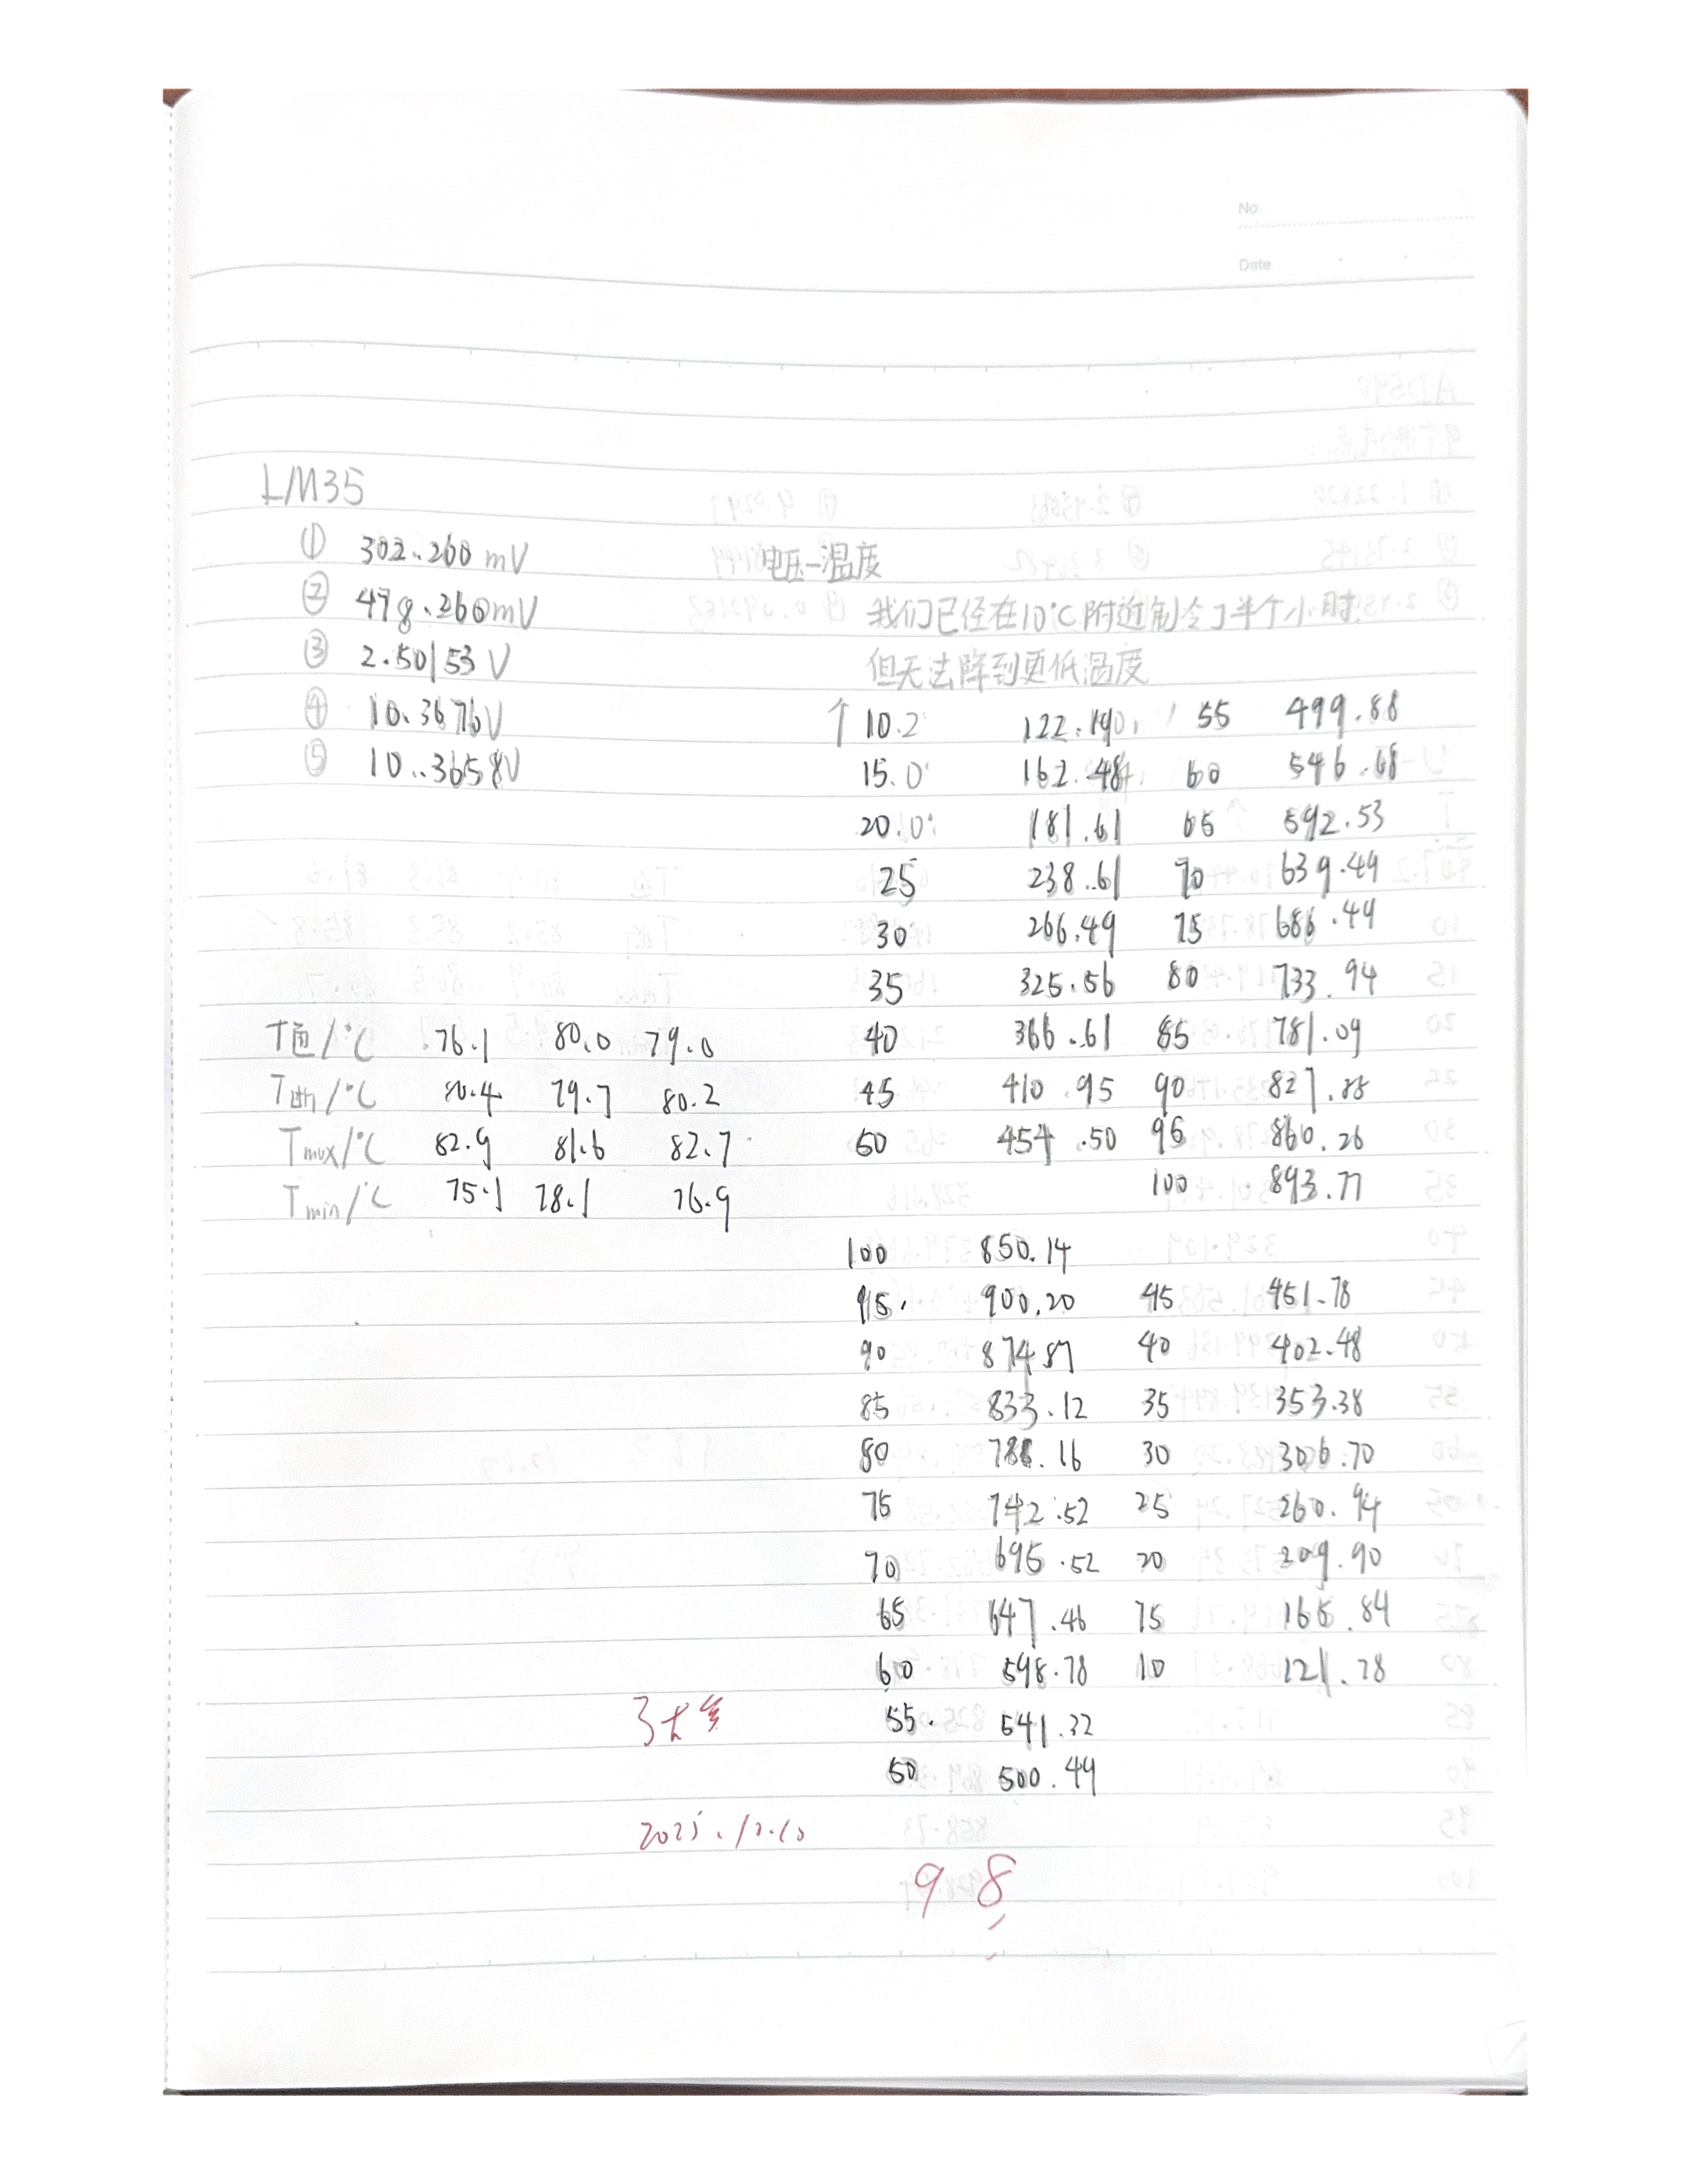
\includegraphics[width=0.6\textwidth]
    {8.1.png} 
    \caption{扫描页}
    \label{8.1} 
  \end{figure}
  
\end{document}